\documentclass{beamer}

\usepackage[utf8]{inputenc}
\usepackage[T1]{fontenc}
\usepackage[T1]{tipa}

\title{Frequency-tuned Salient Region Detection}
\subtitle{Radhakrishna Achanta, Sheila Hemami, Francisco Estrada, and Sabine Süsstrunk}
\author{Alexander Höreth and Sebastian Höffner}
\institute{Institute of Cognitive Science\\University of Osnabrück}
\date[Nov 7, 2016]{I know what you are looking at! -- Gaze Prediction, November 7, 2016}
\subject{Gaze Prediction}

\def\colorful#1{{\usebeamercolor[fg]{enumerate item}#1}}

\bibliographystyle{plain}

\begin{document}

\frame{\titlepage}


\section{Introduction}

\begin{frame}
    \frametitle{Introduction}
    \begin{itemize}
        \item improved image segmentation algorithm
        \item saliency driven
        \item uses properties of lab color space
    \end{itemize}
\end{frame}


\section{Algorithm}

\begin{frame}
    \frametitle{Algorithm}
    \begin{enumerate}
        \item Convert input to lab color space
        \item Calculate mean image
        \item Filter input with 5x5 Gaussian kernel ($\sigma = 1.6$, $I_{\omega}$
        \item $I_S = I_{\mu} - I_{\omega}$
        \item Euclidean distance of $I_S$ yields $S$
        \item Perform mean-shift segmentation
        \item Calculate threshold $\theta = 2S_{\mu}$
        \item Combine mean-shift result with $S$, applying $\theta$
    \end{enumerate}
\end{frame}

\begin{frame}
    \frametitle{Convert to lab color space}
    \begin{figure}
        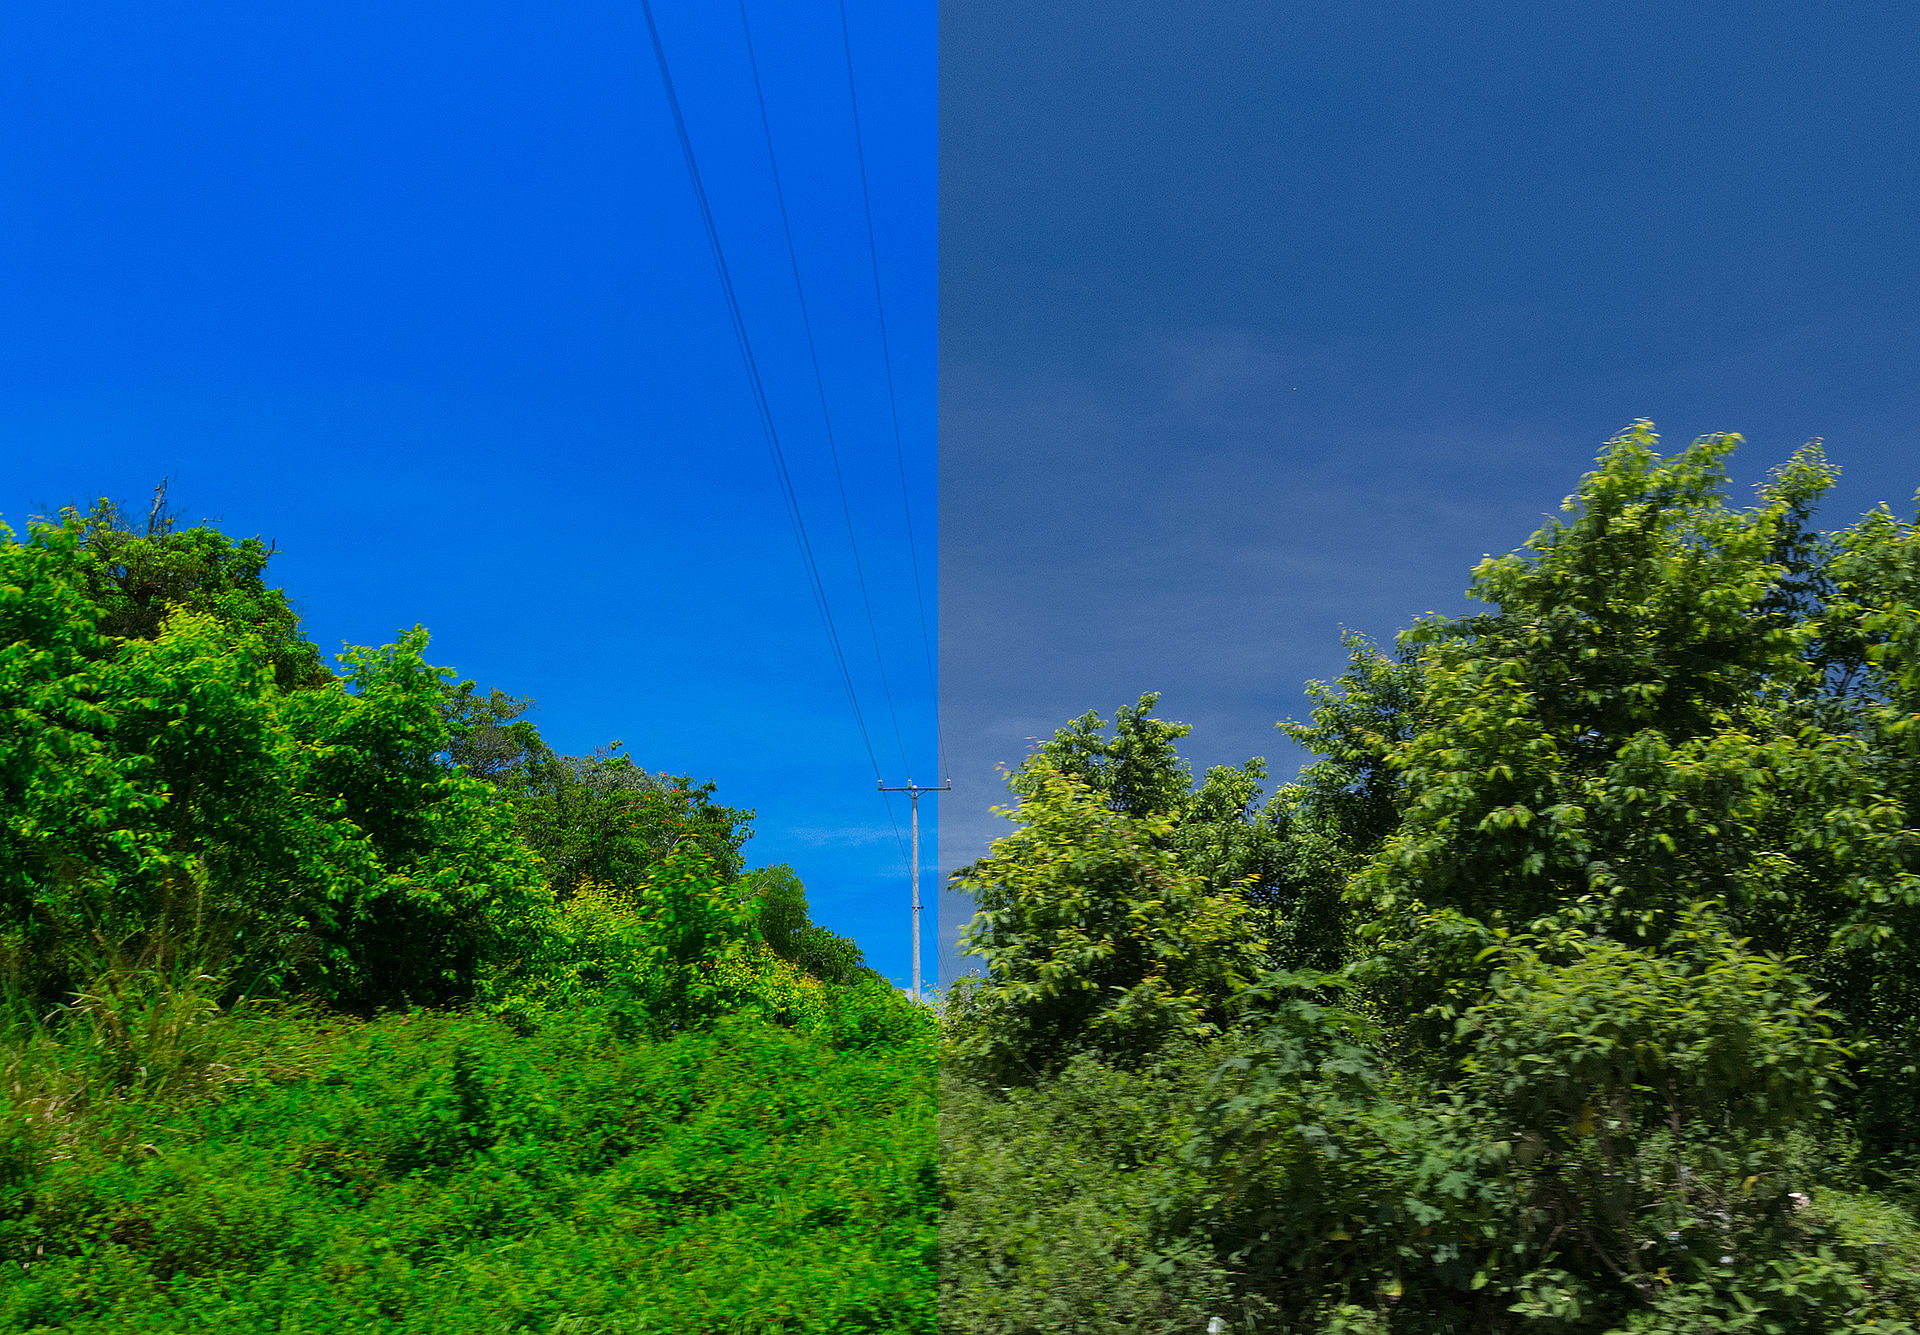
\includegraphics[width=.9\textwidth]{report-images/Example_of_LAB_color_enhancement.jpg}
        \caption{Lab color space conversion. Left Lab, right RGB\@. Image: wikipedia}
    \end{figure}
\end{frame}

\begin{frame}
    \frametitle{Saliency algorithm}
    \begin{figure}
        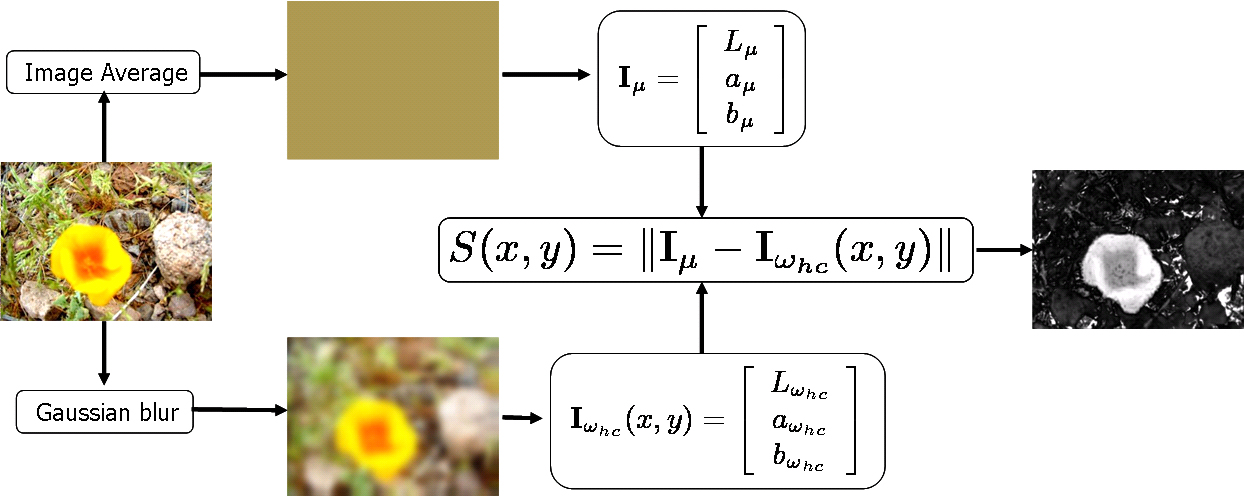
\includegraphics[width=.9\textwidth]{report-images/SaliencyAlgo.jpg}
        \caption{Saliency computation schema. Image: {http://ivrlwww.epfl.ch/supplementary\_material/RK\_CVPR09/}}
    \end{figure}
\end{frame}

\begin{frame}
    \frametitle{Algorithm and Intermediate results}
    \begin{figure}
        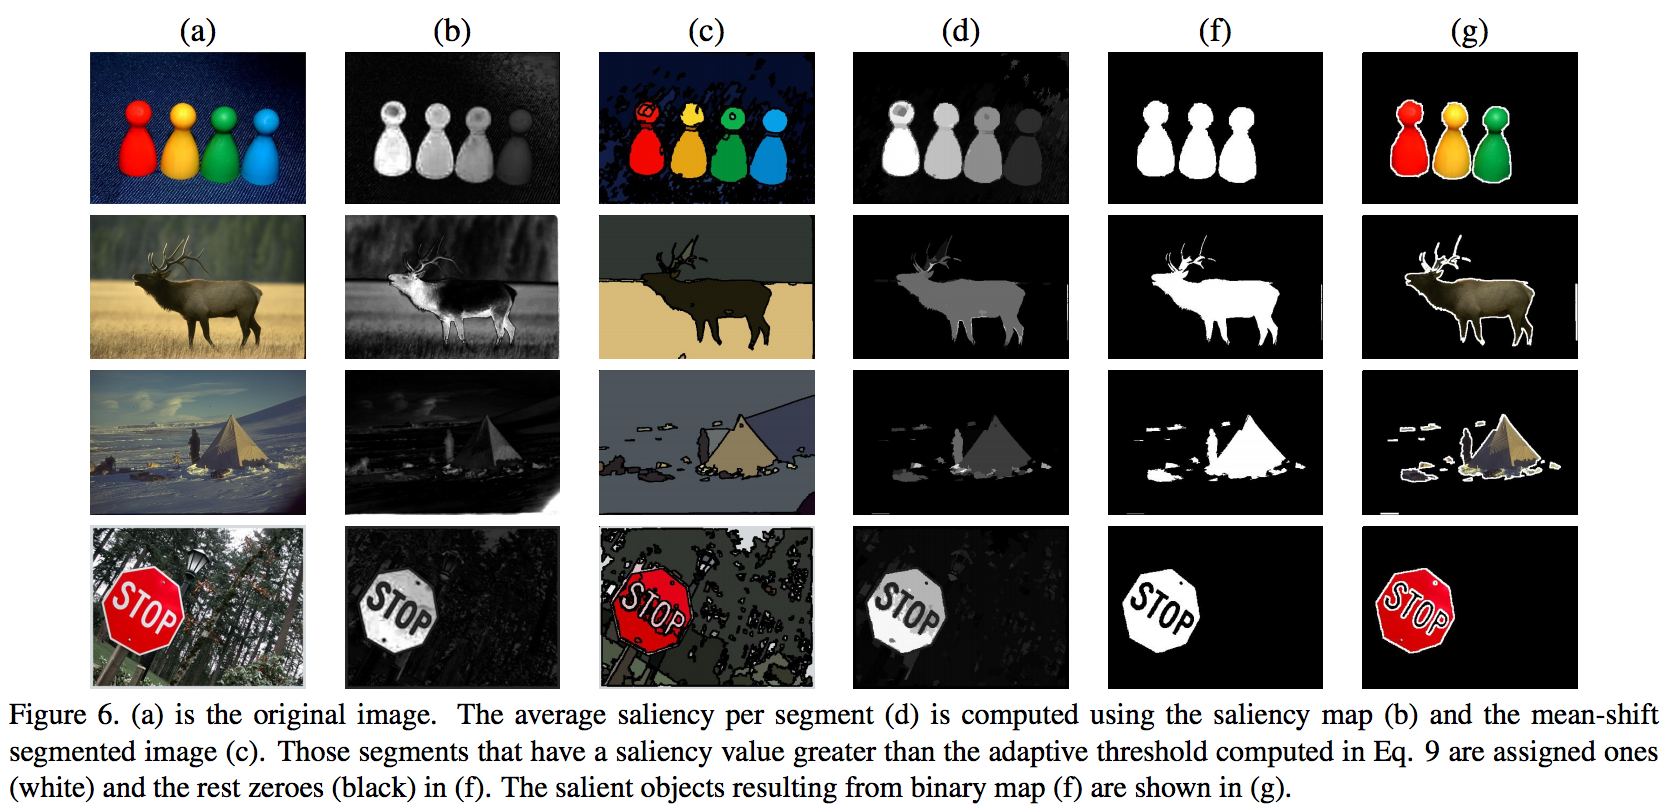
\includegraphics[width=.9\textwidth]{report-images/intermediate_results.png}
        \caption{Intermediate and final results\cite{achanta}.}
    \end{figure}
\end{frame}


\section{Results}

\begin{frame}
    \frametitle{Results/Comparisons}
    \begin{figure}
        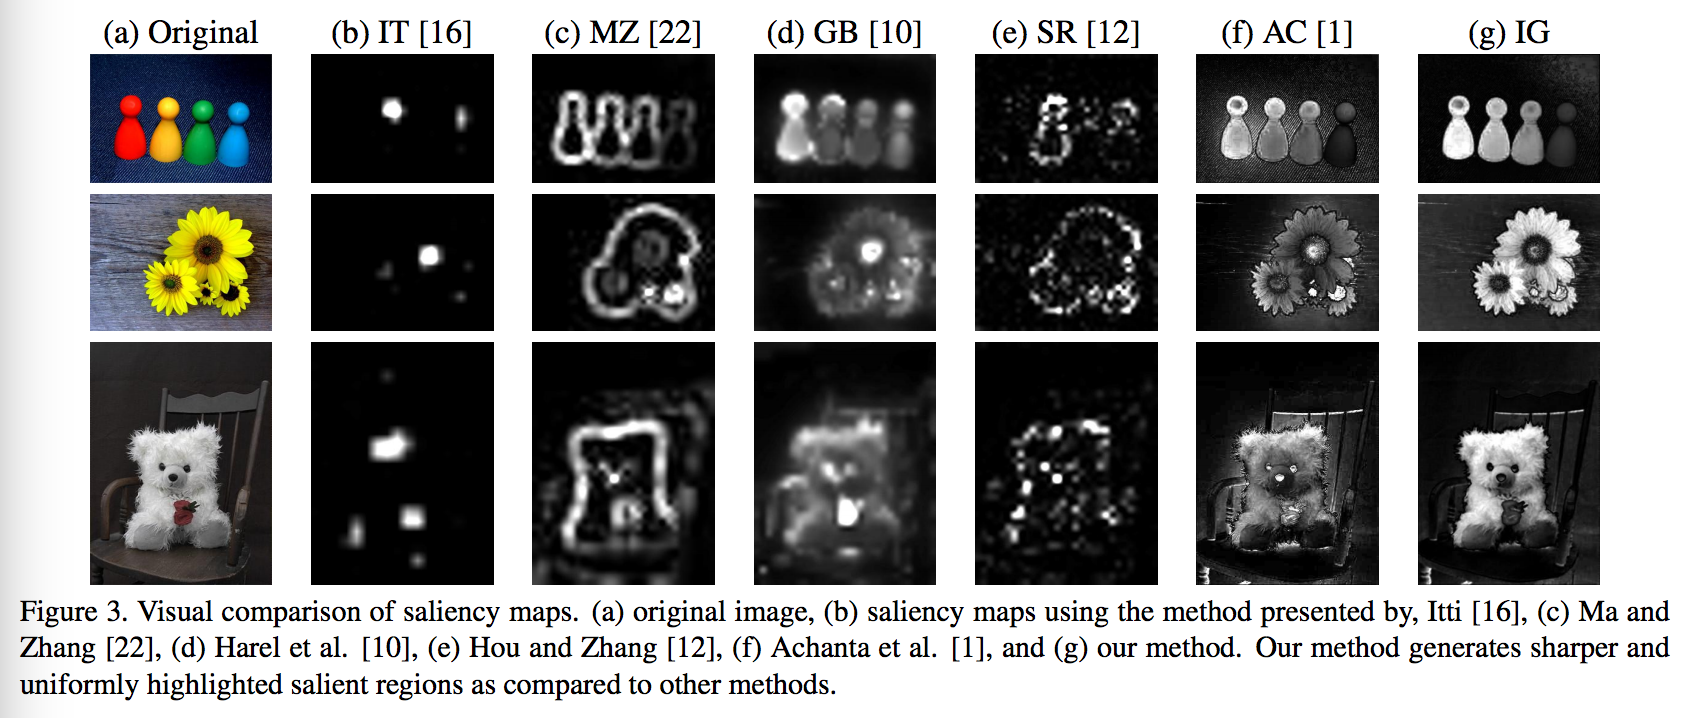
\includegraphics[width=.9\textwidth]{report-images/results.png}
        \caption{Final results and comparisons\cite{achanta}.}
    \end{figure}
\end{frame}


\section{Application}

\begin{frame}
    \frametitle{Own application}
    \begin{itemize}
        \item no mean-shift segmentation
        \item only matlab version, which is only proof of concept
    \end{itemize}
\end{frame}

\begin{frame}
    \frametitle{Own application}
    \begin{columns}
        \column{.45\linewidth}
            \centering
            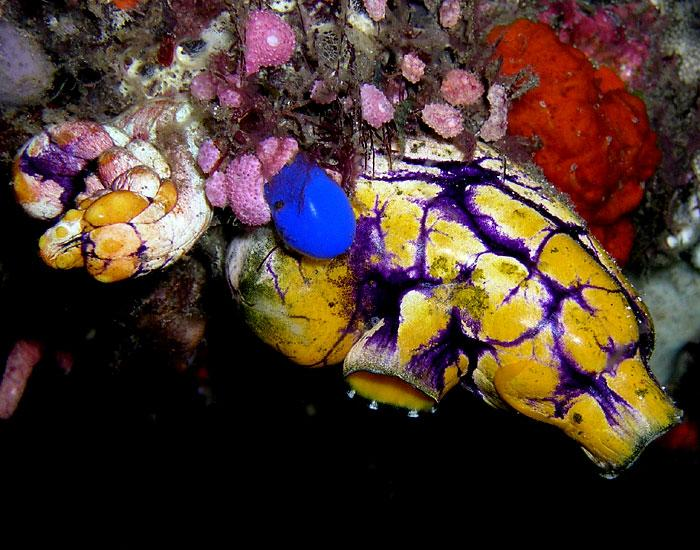
\includegraphics[width=0.95\textwidth]{report-images/Polycarpa_Nick_Hobgood.jpg}
        \column{.45\linewidth}
            \centering
            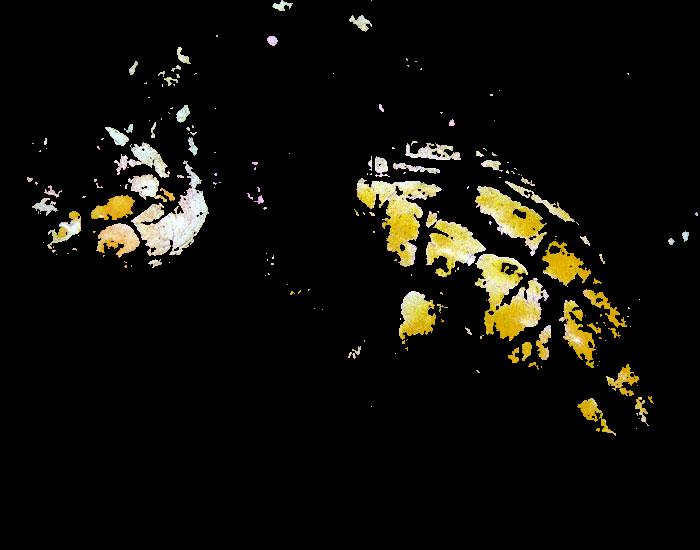
\includegraphics[width=0.95\textwidth]{report-images/thresh_Polycarpa_Nick_Hobgood.jpg}
    \end{columns}
\end{frame}

\begin{frame}
    \frametitle{Own application}
    \begin{columns}
        \column{.45\linewidth}
            \centering
            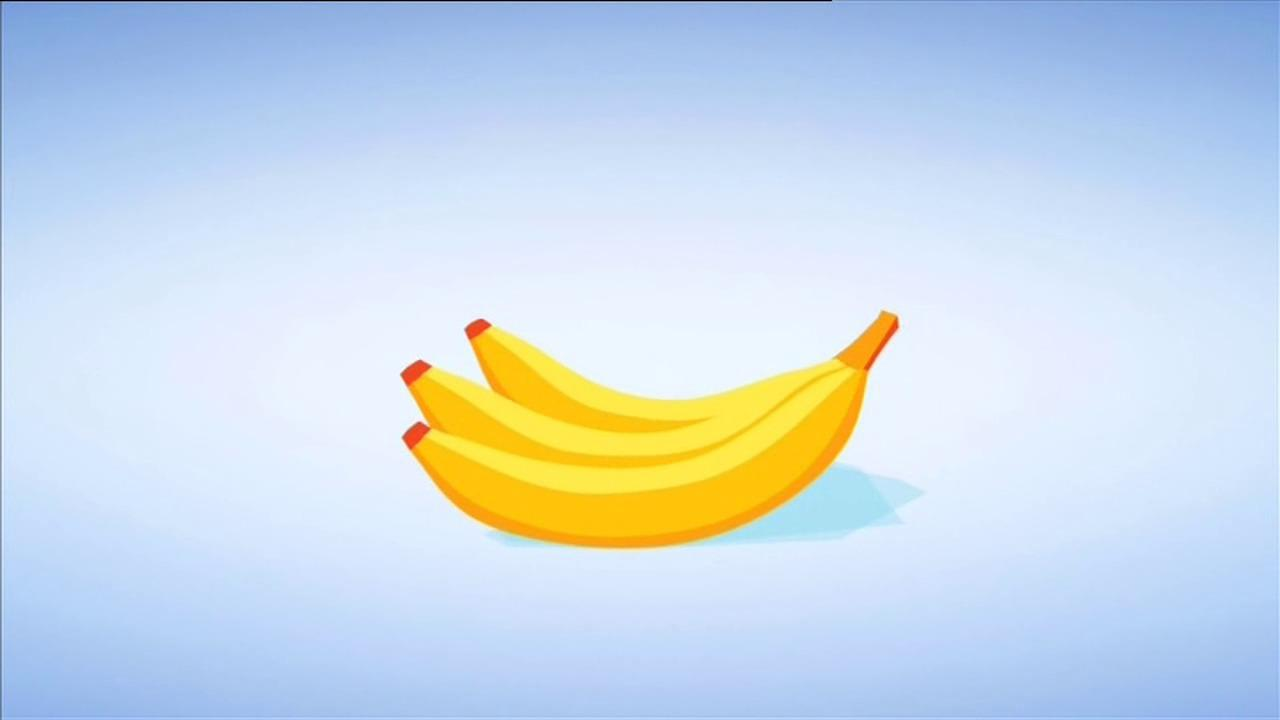
\includegraphics[width=0.95\textwidth]{report-images/a_comm_0088.jpg}
        \column{.45\linewidth}
            \centering
            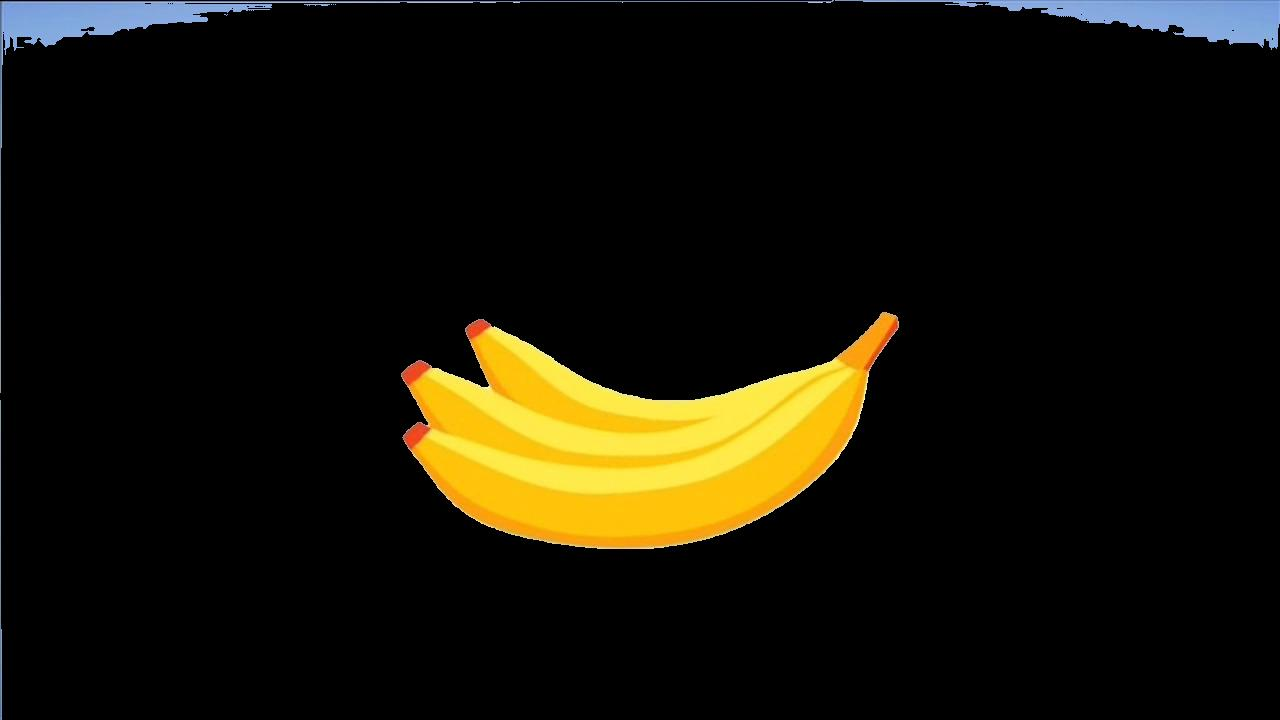
\includegraphics[width=0.95\textwidth]{report-images/thresh_a_comm_0088.jpg}
    \end{columns}
\end{frame}

\begin{frame}
    \frametitle{Own application}
    \begin{columns}
        \column{.45\linewidth}
            \centering
            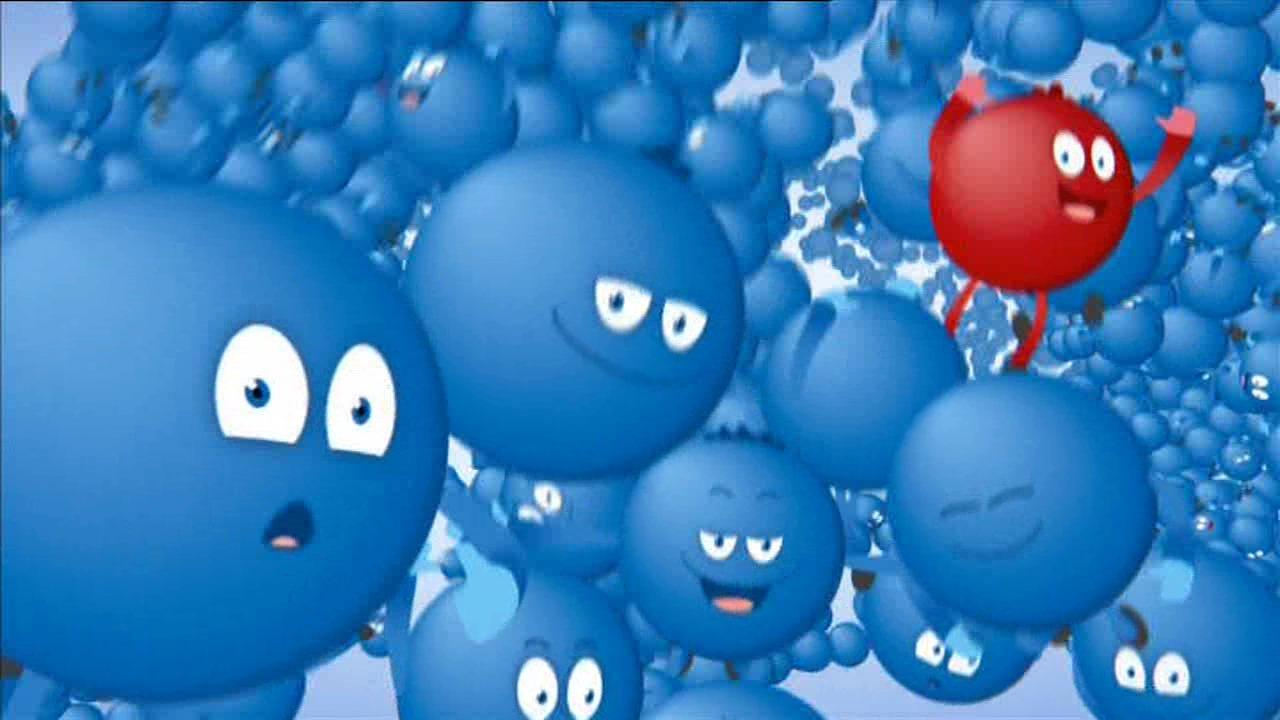
\includegraphics[width=0.95\textwidth]{report-images/a_comm_0225.jpg}
        \column{.45\linewidth}
            \centering
            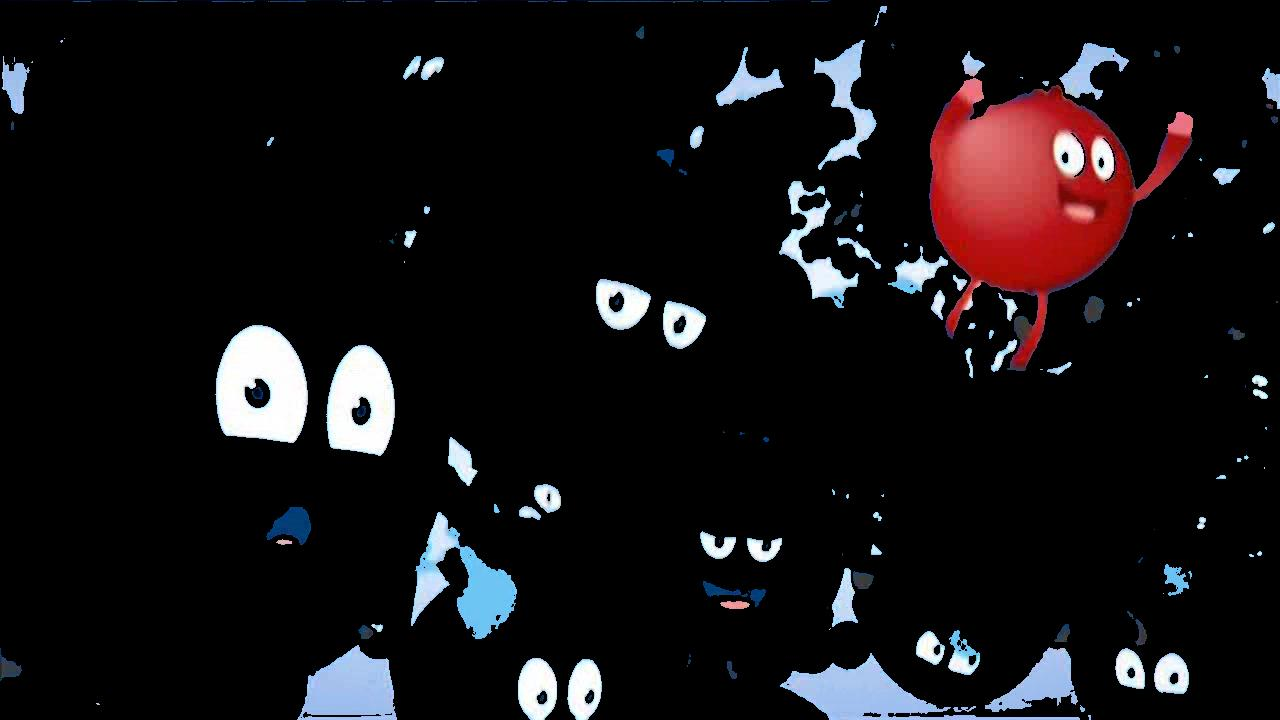
\includegraphics[width=0.95\textwidth]{report-images/thresh_a_comm_0225.jpg}
    \end{columns}
\end{frame}

\begin{frame}
    \frametitle{Own application}
    \begin{columns}
        \column{.45\linewidth}
            \centering
            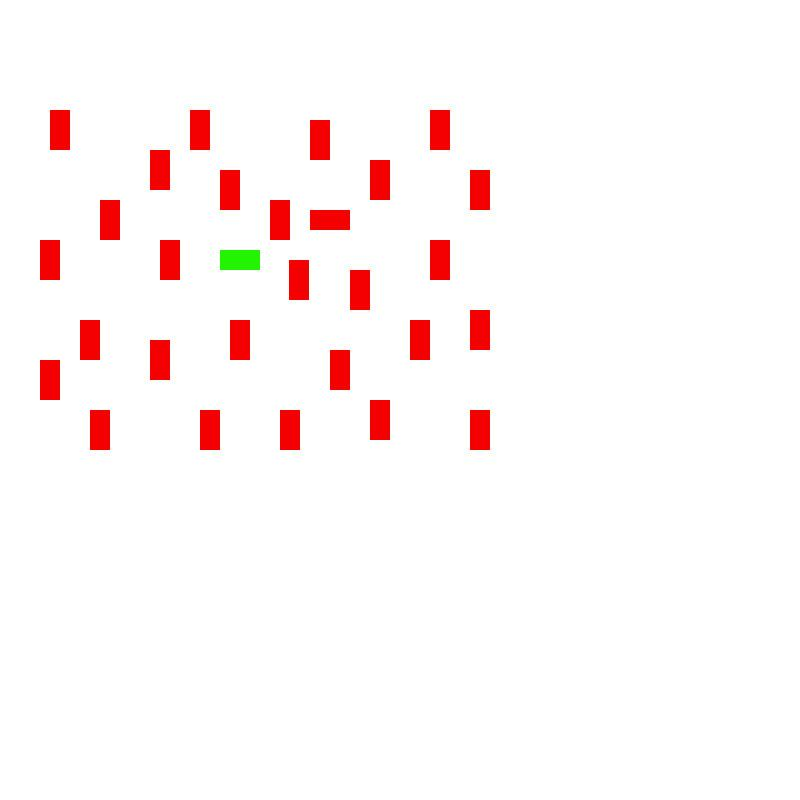
\includegraphics[width=0.95\textwidth]{report-images/vst-04.jpg}
        \column{.45\linewidth}
            \centering
            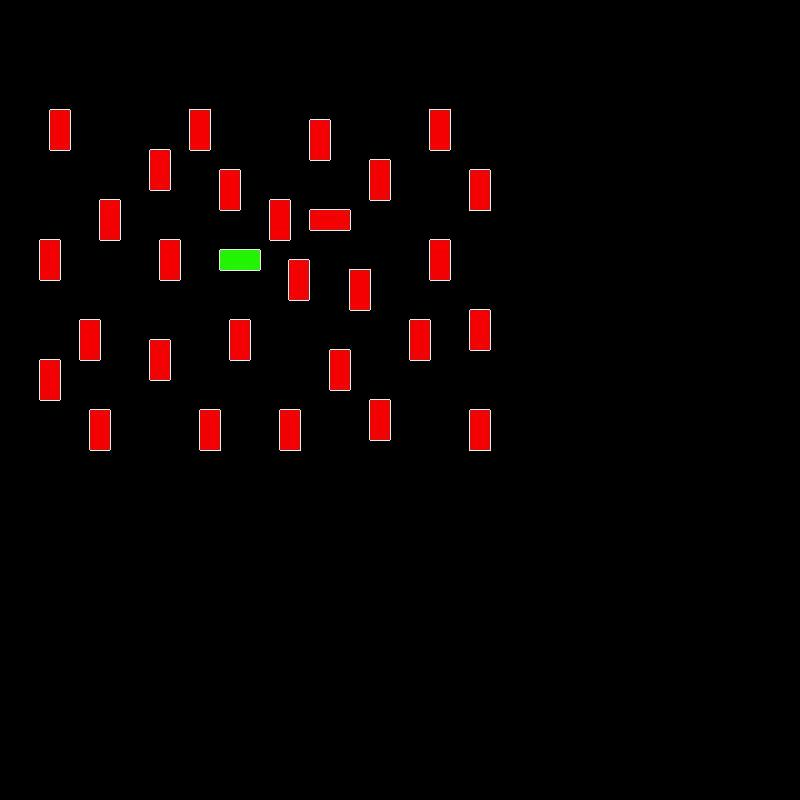
\includegraphics[width=0.95\textwidth]{report-images/thresh_vst-04.jpg}
    \end{columns}
\end{frame}

\begin{frame}
    \frametitle{Own application}
    \begin{columns}
        \column{.45\linewidth}
            \centering
            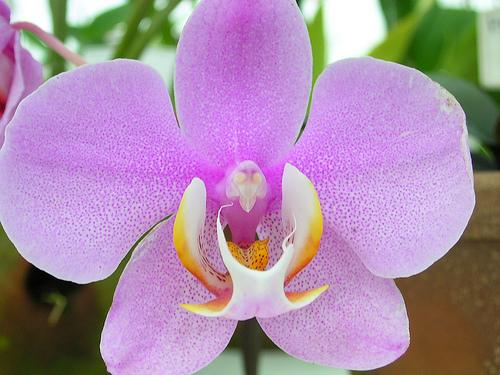
\includegraphics[width=0.95\textwidth]{report-images/3555690726_4d876d7195.jpg}
        \column{.45\linewidth}
            \centering
            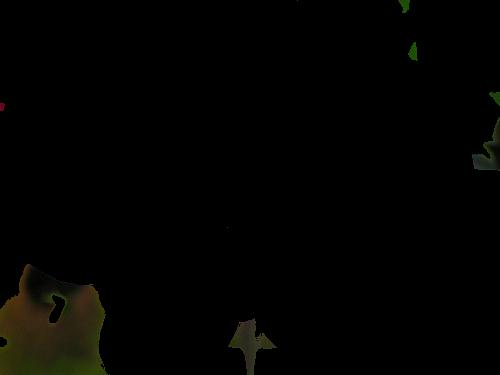
\includegraphics[width=0.95\textwidth]{report-images/thresh_3555690726_4d876d7195.jpg}
    \end{columns}
\end{frame}


\section{Trivia}

\begin{frame}
    \frametitle{Ascidiacea (Sea Squirt)}
    \begin{columns}
        \column{.45\linewidth}
            \centering
            \begin{figure}
                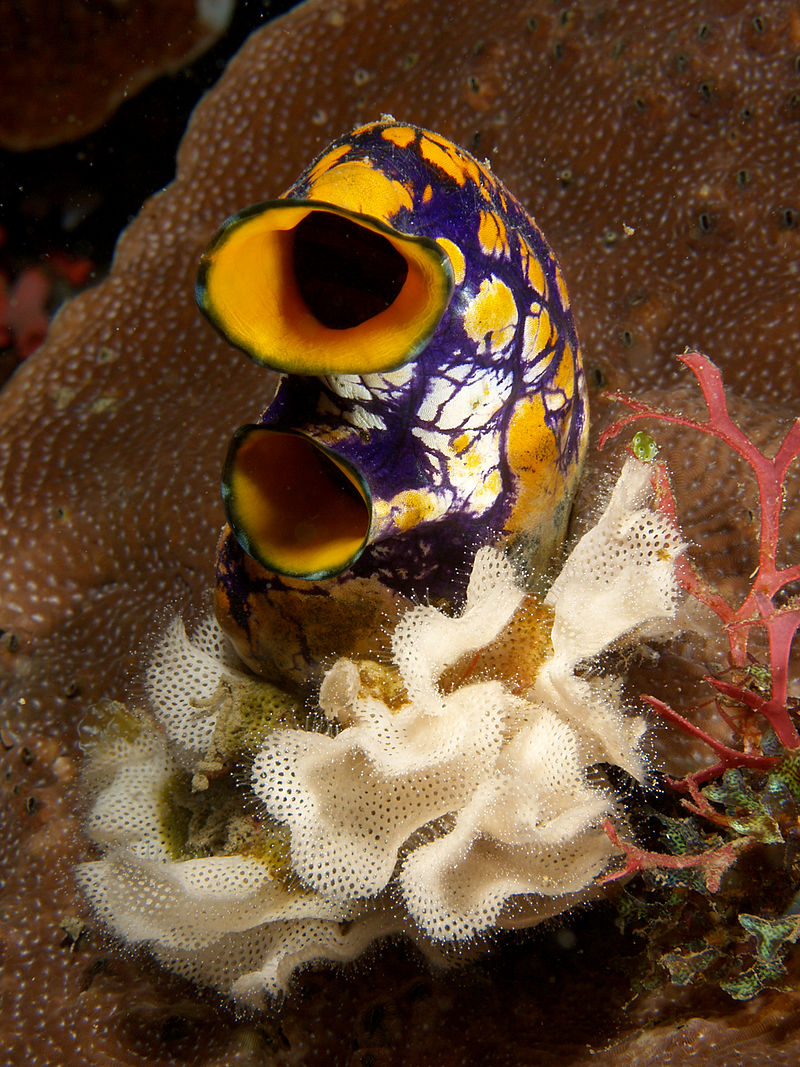
\includegraphics[width=0.95\textwidth]{report-images/Polycarpa_aurata.jpg}
                \caption{Polycarpa aurata, a seasquirt. Image: Nhobgood via wikipedia}
            \end{figure}
        \column{.45\linewidth}
            \begin{itemize}
                \item swim around until they touch down
                \item consume their ``brain'' (metamorphosis removes cerebral ganglion to build digestive system)
                \item often appear in colonies
                \item can reproduce sexually and asexually
                \item some species are used as food all over the world
            \end{itemize}
    \end{columns}
\end{frame}


\section{References}

\begin{frame}
    \frametitle{References}
    \bibliography{report.bib}
\end{frame}

\end{document}
